\chapter{The Sandpile Model}
\thispagestyle{fancy}

\section{Bak-Tang-Wiesenfeld Model}

The classical sandpile model represents a cellular automation describing a dynamical system following certain rules that can be described as follows.

The field/lattice, which is chosen to be two-dimensional, represents a sandpile. Each site on the lattice has a certain value $z$ that intuitively represents the height or slope of the sandpile at certain position described with the coordinates $x$ and $y$. At each time step, a number of grains of sand is placed on top of a random site, which increases its value by a given value, e.g. one. If the value of the site exceeds a critical value $z_c$ (e.g. three), the site collapses/topples and its grains are evenly distributed to its neighbours.

In certain cases some of the adjascent sites will exceed the critical value too and the toppling process will continue until an equilibrium state is again reached. This series of collapsing sites is clasically described as an avalanche. The next grain is not placed until the equilibrium state is reached, meaning that the time scale of the random grain placement and of the development of avalanches are decoupled.

The classical model description can mathematically be represented as follows.

Initially, the lattice is empty:
\[
z(x,y) = 0 \quad\forall x, y
\]
Then, the value of a random site $x,y$ is increased:
\[
z(x,y) \to z(x_r,y_r) + 1
\]
If its value exceeds the critical value $z_c=3$, then it topples and distributes its grains to its neighbours:
\[
\begin{aligned}
z(x,y) \overset{?}{>} 3 \Rightarrow & z(x,y) \to z(x,y)-4 \\
 & z(x\pm 1,y) \to z(x\pm 1,y)+1 \\
 & z(x,y\pm 1) \to z(x,y\pm 1)+1 \\
\end{aligned}
\]

Clearly, many variations of the described model can be considered and can produce different results. The classical sandpile model, as originally described by Per Bak, Chao Tang and Kurt Wiesenfeld, represents the starting point of any further investigations considered in this paper.

\section{Parameters}
The behavior of the model is analysed dependent on different parameters such as:
\begin{itemize}
 \item lattice size
 \item number of dimensions of lattice
 \item mass conservation, i.e. if the number of grains removed from a collapsed site is equal to the sum of grains its neighbour sites received
 \item boundary conditions, see below
 \item etc.
\end{itemize}
Different types of boundary conditions can be thought of:
\begin{itemize}
 \item open: If a site near the border topples, some of its grains leave the system (mass is lost).
 \item closed: Near-border site does not fully collapse, but keeps the grains that would fall off in an open case.
 \item periodic: The system has no boundaries, i.e. toppling near the border is ``wrapped over''.
 \item mixed: E.g. the lattice is periodic in one dimension and has open boundaries in another dimension.
\end{itemize}
Figure \ref{pics:boundary} illustrates the first three basic types of boundary conditions.

\begin{figure}[!htpb]
\centering
\includegraphics[width=0.5\textwidth]{pics/pic4_boundary.pdf}
\caption[]{Effect of different types of boundary conditions on a sample lattice (1): open (2), closed (3) and periodic (4)}
\label{pics:boundary}
\end{figure}

\section{Abelian Model}
One important property which can be used to categorize different sandpile models is whether they behave in a commutative or \emph{abelian} way. In particular, this can be applied to the development of avalanches in the model described above: The question posed here is, whether an equilibrium state resulting from an avalanche depends on the way the avalanche is calculated. More precisely, it can be shown that any avalanche, being a sequence of topplings, always results in the same equilibrium state i.e. does not depend on the order, in which the topplings occur. The mathematical proof of this hypothesis is nicely presented in \cite{sandpile_math}.

To illustrate this practical but not necessarily obvious fact, a sample 4x4-field with one active site is considered (see figure \ref{pics:abelian}). At step (2), two different sites simultaneously become active, therefore creating a ``choice'', which site to topple first. Depending on such choices, different sequences of topplings occur, but all lead to the same equilibrium state.

\begin{figure}[!htpb]
\centering
\includegraphics[width=\textwidth]{pics/pic1_abelian.pdf}
\caption[]{Demonstration of the abelian property: six different orders of topplings all lead to the same equilibrium state. The sites circled red indicate sites that have just become active, those circled black have just collapsed. Here, continuous boundary conditions have been used.}
\label{pics:abelian}
\end{figure}
